\documentclass[12pt,a4paper]{article}
\usepackage[UTF8]{ctex}     %先引入ctex
\usepackage[utf8]{inputenc} %再引入inputenc
\usepackage{graphicx}
\usepackage{geometry}
\usepackage{xcolor}
% \usepackage{lazylatex}
\usepackage{amsmath}
\usepackage{enumerate}
\usepackage{caption}
\usepackage{listings}
\captionsetup[lstlisting]{labelfont=bf,justification=justified}

\usepackage{tikz}
\usepackage{pgfplots}
\pgfplotsset{compat=1.17}
\usepackage{appendix}

\graphicspath{{img/}}
% 边距
\geometry{left=2.0cm,right=2.0cm,top=2.0cm,bottom=3.0cm}
% 大题
\newenvironment{problems}{\begin{list}{}{\renewcommand{\makelabel}[1]{\textbf{##1}\hfil}}}{\end{list}}
% 小题
\newenvironment{steps}{\begin{list}{}{\renewcommand{\makelabel}[1]{##1.\hfil}}}{\end{list}}
% 答
\providecommand{\ans}{\textbf{答}:~}
% 解
\providecommand{\sol}{\textbf{解}.~}

\usepackage[colorlinks,linkcolor=blue]{hyperref}
\usepackage{bookmark}
\providecommand{\code}[2]{\lstinputlisting[language=#2,caption=\href{run:#1}{\ttfamily #1}]{#1}}
\providecommand{\img}[1]{\includegraphics[width=0.88\textwidth]{#1}}

% listings
\definecolor{grey}{rgb}{0.8,0.8,0.8}
\definecolor{darkgreen}{rgb}{0,0.3,0}
\definecolor{darkblue}{rgb}{0,0,0.3}
\lstset{%
    % numbers=left, %行号
    % numberstyle=\tiny\color{grey},
    showstringspaces=false,
    showspaces=false,%
    tabsize=4,%
    frame=shadowbox,%
    basicstyle={\ttfamily\scriptsize},%
    keywordstyle=\color{blue!80!black}\bfseries,%
    identifierstyle=,%
    commentstyle=\color{green!50!blue}\itshape,%
    stringstyle=\color{green!50!black},%
    rulesepcolor=\color{gray!20!white},
    breaklines,
    columns=flexible,
    extendedchars=false,
    %mathescape=true,
    language=c,
}

\begin{document}
\title{\normalsize \underline{操作系统(D)}\\\LARGE 项目 8}
\author{李子龙 518070910095}
\date{\today}
\maketitle

\textbf{设计虚拟内存管理器}

\begin{problems}
    \item[1.] \textbf{起步}
    
    首先将测试用的地址写入 trial.txt,以测试 \verb"addext" 内存地址分析模块的正确性。
    \code{src/trial.txt}{}

    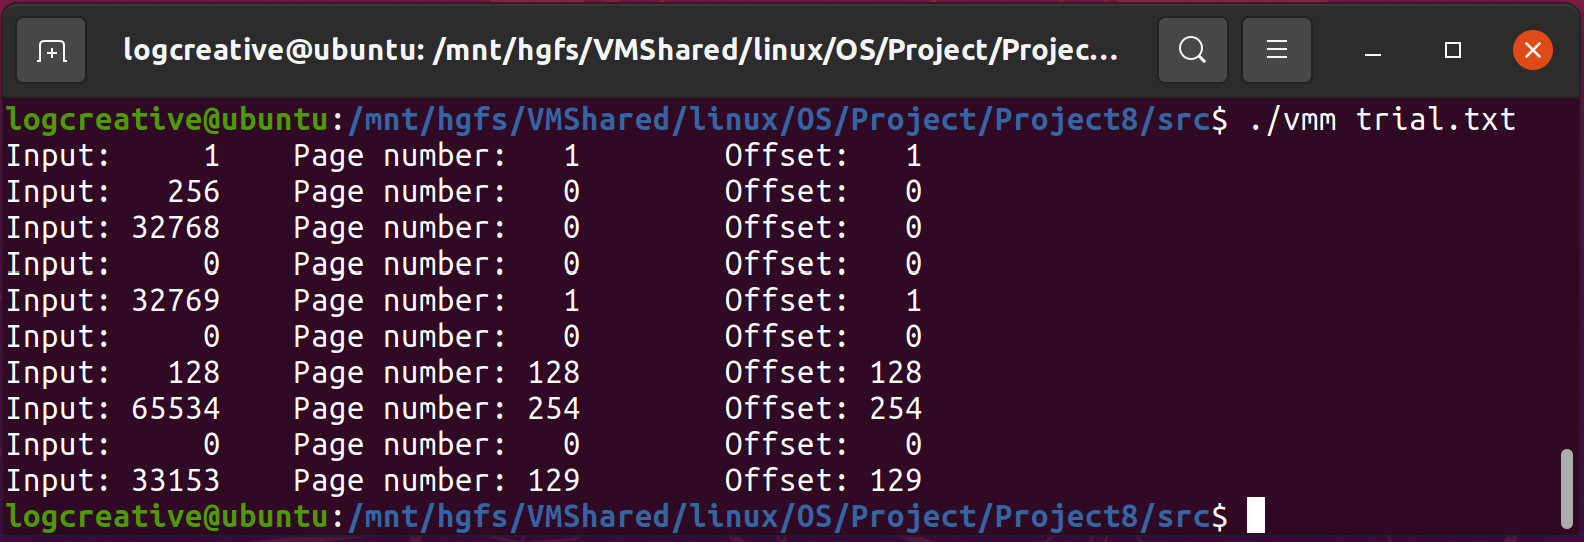
\includegraphics[width=0.88\textwidth]{trial.png}

    定义地址结构和地址提取器如下:
    \code{src/addext.h}{c}
    \code{src/addext.c}{c}
    
    \item[2.] \textbf{处理页面错误}
    
    接着,先不考虑 TLB,只使用页表。将输出结果与正确参考比较,结论是正确:

    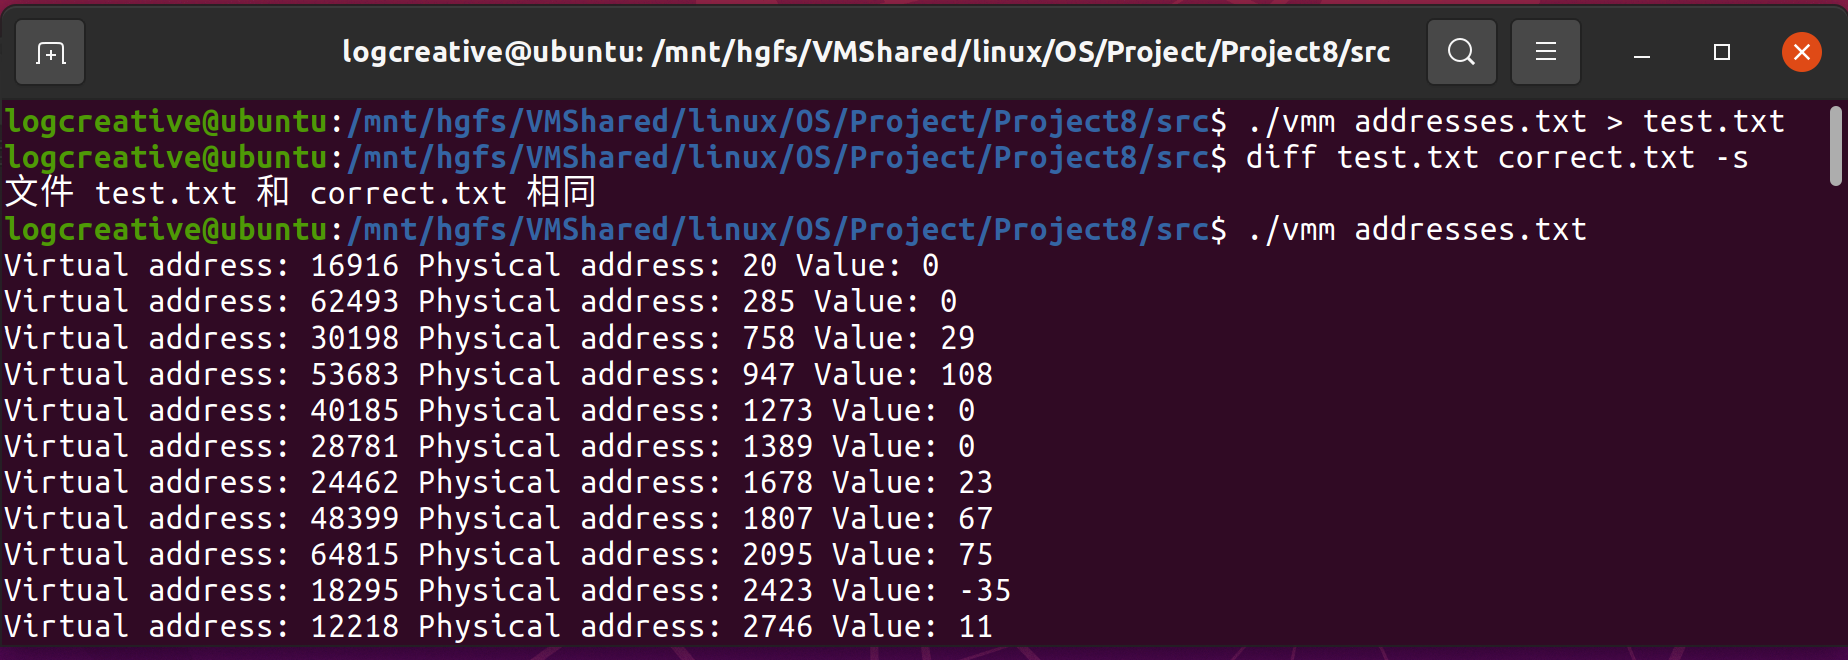
\includegraphics[width=0.88\textwidth]{pagetab.png}

    首先对输入流分析,在 \verb"main" 函数里的情形如下:
    \begin{lstlisting}[language=c]
    while(fgets(addline, MAXLINE, addfile)!=NULL){
        int rline = atoi(addline);
        add viradd = addext(rline);
        add phyadd = getPhyAdd(viradd);
        fprintf(stdout, "Virtual address: %d Physical address: %d Value: %d\n", 
            getAdd(viradd), getAdd(phyadd), getValue(phyadd));
    }
    \end{lstlisting}

    获取值是直接从内存中获得对应位置的值:
    \begin{lstlisting}[language=c]
int getValue(add _phyadd) {
    return mem[_phyadd.number][_phyadd.offset];
}
    \end{lstlisting}

    其中 \verb"mem" 是用 \verb"char" 存储的:
    \code{src/memory.h}{c}

    当前只使用页表是不需要考虑 TLB 的获取物理地址的函数如下:
    \begin{lstlisting}[language=c]
add getPhyAdd(add _inadd) {
    add phyadd;

    if (!page_table[_inadd.number][1])
        handle_pagefault(_inadd.number);

    phyadd.number = page_table[_inadd.number][0];
    phyadd.offset = _inadd.offset;
    return phyadd;
}
    \end{lstlisting}

    一旦有页面错误就会触发对应的函数,将内容存放到内存中去:
    \begin{lstlisting}[language=c]
void handle_pagefault(int page_number) {
	int frame_number = read_frame(page_number);
	page_table[page_number][0] = frame_number;
	page_table[page_number][1] = 1;
}
    \end{lstlisting}

    由于现在的内存充足,帧码直接用静态变量 \verb"frame_number" 递增存储。
    \begin{lstlisting}[language=c]
int read_frame(int page_number) {
	static int frame_number = 0;

	FILE* backstore;
	if ((backstore = fopen("BACKING_STORE.bin", "rb")) == NULL) {
		fprintf(stderr, "Empty file storage!\n");
		return -1;
	}

	int frame_number_ = frame_number++;
	long pos = page_number * FRAMESIZE;
	fseek(backstore, pos, SEEK_SET);
	fread(mem[frame_number_], sizeof(char), FRAMESIZE, backstore);
	fclose(backstore);

	return frame_number_;
}
    \end{lstlisting}
    这里使用了二进制文件读取的方式复制到内存中去。

    \item[3.] \textbf{使用 TLB}
    
    使用 \verb"test.sh" 脚本进行相同的测试后,结果仍然是一致的。
    \code{src/test.sh}{}
    
    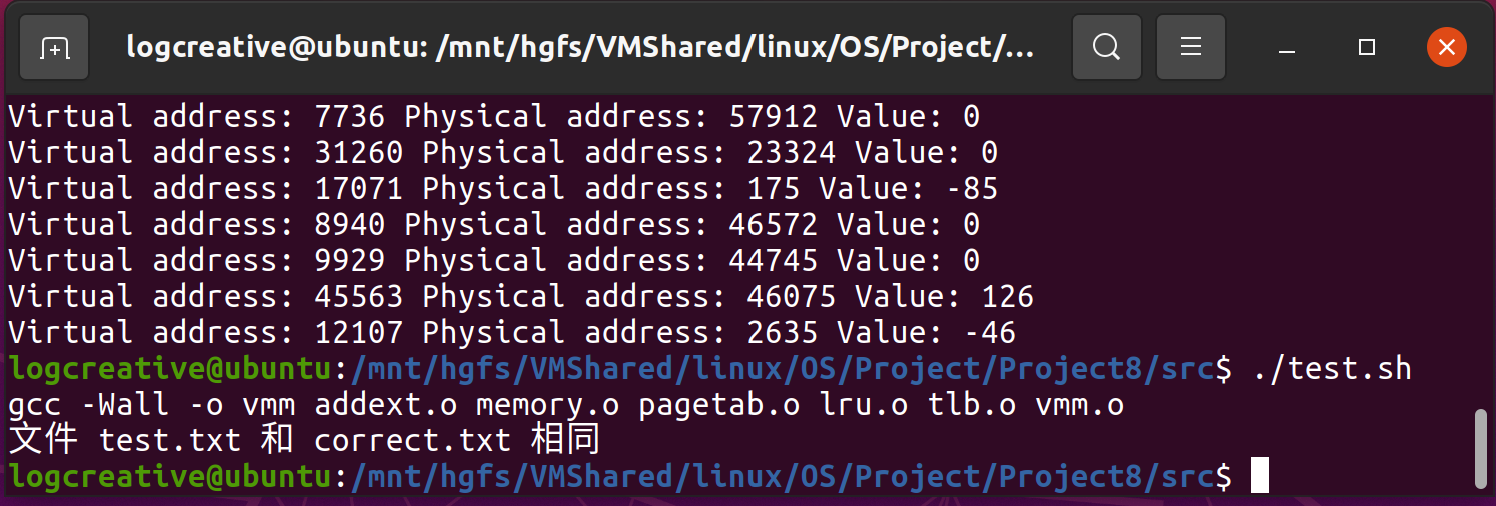
\includegraphics[width=0.88\textwidth]{tlb.png}

    首先,输入流分析被重定向到 TLB 对应的接口。
    \begin{lstlisting}[language=c]
add getPhyAdd(add _inadd) {
    add phyadd;

    phyadd.number = tlb_search(_inadd.number);
    phyadd.offset = _inadd.offset;
    
    return phyadd;
}
    \end{lstlisting}

    TLB 由 16 个内存块组成。
    \code{src/tlb.h}{c}

    而最主要的 \verb"tlb_search" 函数首先会尝试 TLB 命中,接着如果是 TLB 未命中,就看需不需要触发页面缺失,然后看是否由空余 TLB 空间用于存储到 TLB 中。如果 TLB 满,就会使用 LRU 算法进行 TLB 置换。
    \code{src/tlb.c}{c}

    对于 TLB 使用状态使用了双向链表式栈存储,记录头 \verb"tlb_head" 和尾 \verb"tlb_tail"。对应的 LRU 操作具有如下定义:
    \code{src/lru.h}{c}

    \begin{itemize}
        \item \verb"search_pop" 将会寻找对应的栈节点,并移除。
        \item \verb"push" 入栈操作。
        \item \verb"bottom_pop" 栈底出栈。
    \end{itemize}

    \code{src/lru.c}{c}

    \item[4.] \textbf{添加统计信息}

    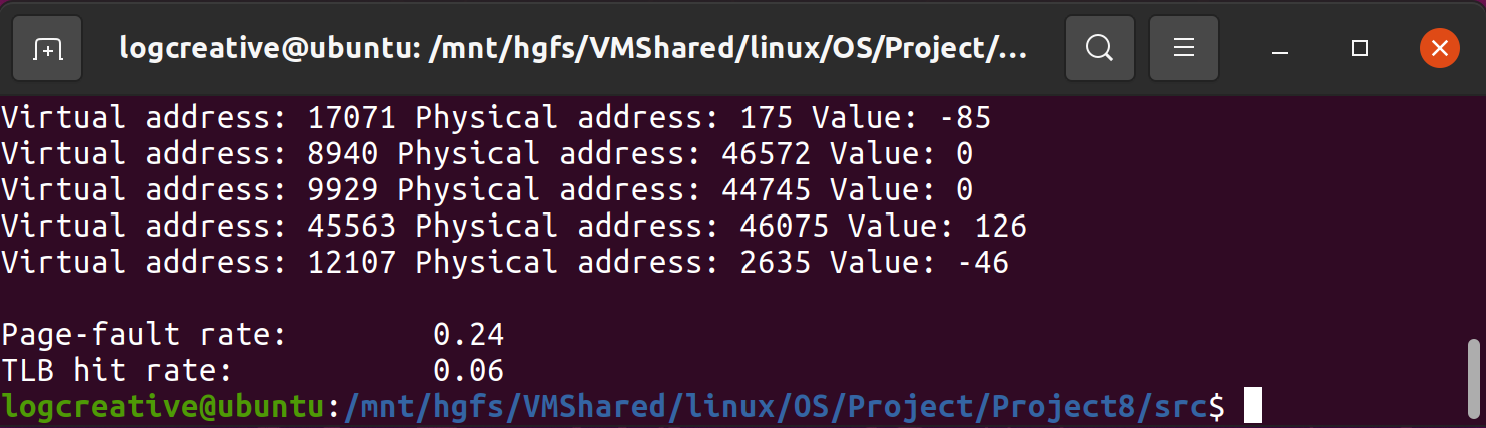
\includegraphics[width=0.88\textwidth]{stat.png}

    添加统计接口,方可在主函数中获得统计信息。添加 \verb"-s" 参数可以显示统计信息。

    \begin{lstlisting}[language=c]
        if(argc==3 && strcmp(argv[2],"-s")==0)
            fprintf(stdout, "\nPage-fault rate:\t%.2f\nTLB hit rate:\t\t%.2f\n", get_pagefault_rate(), get_tlbhit_rate());
    \end{lstlisting}

    \item[5.] \textbf{页面置换}
    
    将内存帧数设定为 128 后,结果如下:

    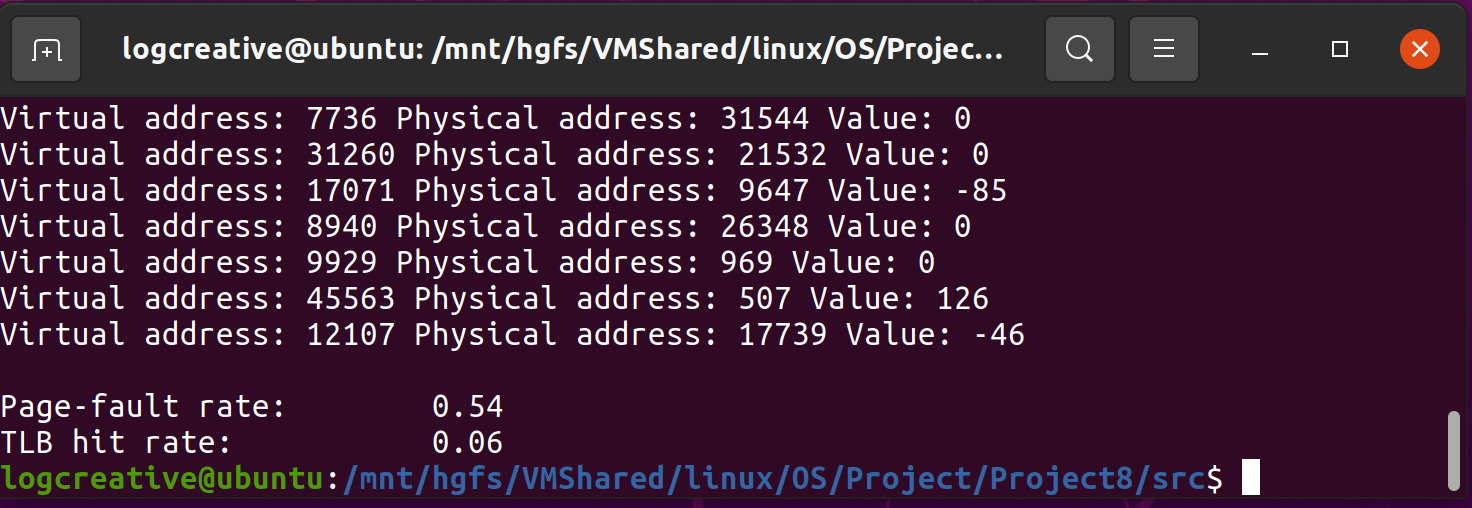
\includegraphics[width=0.88\textwidth]{pagerepl.png}

    当下的内存关于读取帧的定义发生了改变,采用 LRU 算法进行页面置换。
    \code{src/memory.h}{c}
    \code{src/memory.c}{c}

    对于发生了页面置换后的帧 $N$,将会返回
    \begin{equation*}
        -N-1
    \end{equation*}
    标识替换。

    获取内存值时,将会对访问后的帧对应的内存访问栈进行更新。注意,当页面置换已经弹出该帧时,\verb"search_pop" 将会什么都不做。

    \code{src/pagetab.h}{c}
    \code{src/pagetab.c}{c}

    对应的置换信息将会传递页表中,采用下面的方式复原
    \begin{equation*}
        -(-N-1)-1 = N
    \end{equation*}

    并从当前的页表中寻找对应的替换帧置为无效。

    \begin{lstlisting}[language=c]
        if (!page_table[page_number][1]) { // page fault
			if (handle_pagefault(page_number)) {	// page replacement
				int frame_number_r = page_table[page_number][0];
				for (int i = 0; i < TLBSIZE; ++i)
					if (TLB[i][2]
						&& TLB[i][1] == frame_number_r)
						TLB[i][2] = 0;
			}
			++page_fault_number;
		}
    \end{lstlisting}

    替换信息将会按照 0-1 返回到 TLB 中,将会寻找当前 TLB 中是否有对应帧的存储信息,如果有将会被置为无效,变成可以被 \verb"hole" 捕捉的 TLB 位置。找不到就什么都不做。

\end{problems}

\begin{appendices}
    \section{Makefile}
    \code{src/Makefile}{}

\end{appendices}

\end{document}